\chapter{Estrategias de planificación de queries}
\label{cap:planificacion}

Nosotros optamos por un enfoque de Wand Heap Compartido para ser usado en los experimentos.

Se habla de enfoque de bloques también.


\section{Estrategias por bloques}
\label{scheduling:fr}

// Se explica

// Esquema de ejecución

// Algoritmo

// Ejemplo de cómo van quedando los bloques



\section{Estrategia \textit{1TQ}}
\label{scheduling:baseline}
Un simple camino para construir un sistema que responda a múltiples consultas simultáneamente usando múltiple hilos de ejecución, es usando estos hilos de manera independiente. Para hacer esto se debe mantener un conjunto de \textit{threads} consumidores que trabajarán en paralelo y se encargarán de resolver las \textit{queries} secuencialmente (una a una) desde una misma cola, esto es lo que en este trabajo se denomina estrategia de Un Thread Por Query (1TQ). En la Figura \ref{fig:1TQ} se puede apreciar el esquema de ejecución en donde cada uno de los procesos genera una petición de alguna consulta en la cola, si quedan \textit{queries} por procesar entonces se le asigna al proceso una consulta que tendrá que resolver de manera secuencial. Se debe tener en cuenta que cada vez que un proceso genera una solicitud de \textit{query}, se bloquea la estructura de datos que contiene las consultas a procesar y luego se procesa la solicitud, de esta forma se asegura un acceso seguro por parte de los distintos \textit{threads}. 

\begin{figure}[H]
\centering
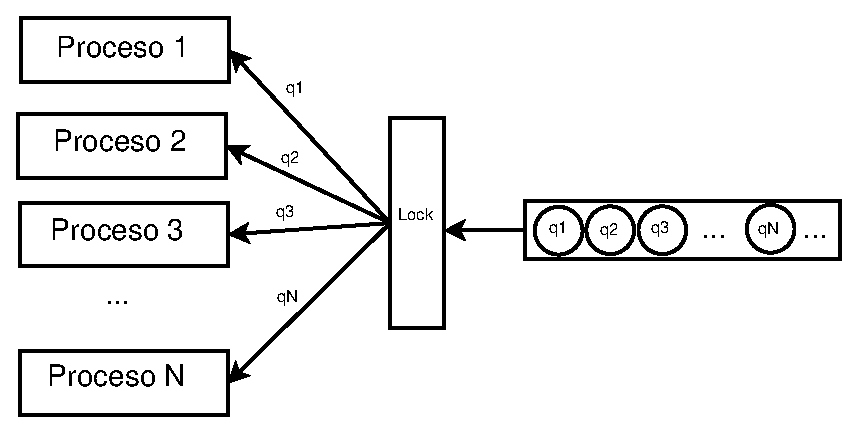
\includegraphics[scale=.75]{images/1TQ.eps}
\caption{Ejemplo de procesamiento estrategia 1TQ}
\label{fig:1TQ}
\end{figure}

Este esquema tiene la ventaja que es simple y fácil de implementar y controlar. Sin embargo, existen sistemas de recuperación de la información como los motores de búsqueda verticales que cuando están ejecutando \textit{batches} de \textit{queries} deben parar su ejecución porque transacciones de escritura han llegado al sistema, y este deben actualizar la información del índice invertido. Solo después de la fase de actualización el sistema es capaz de ejecutar el siguiente \textit{batch} de transacciones de lectura. Al final de cada conjunto de consultas, es posible que algunos hilos de ejecución del sistema finalicen su trabajo y que no tengan más \textit{queries} para procesar, por lo que ellos tienen que esperar que los \textit{threads} restantes finalicen su trabajo antes que el sistema entre en la fase de actualización de su índice invertido o bien, se pase a la ejecución del siguiente \textit{batch} de consultas.
Sin embargo, aunque cada hilo de ejecución está secuencialmente ejecutando una transacción de lectura diferente, algunas de estas operaciones puede tomar un tiempo cosiderable, de esta forma se produce una importante pérdida de eficiencia, aunque la intuición nos dice que esto se puede mitigar con \textit{queries} que requieran poca cantidad de tiempo para ser procesada (trabajos pequeños o \textit{small jobs}). 
En la Figura \ref{fig:small_jobs} queda reflejado lo dicho en el párrafo anterior. Si los trabajos que cada \textit{thread} está ejecutando son pequeños, entonces probablemente la pérdida de trabajo al final de cada \textit{batch} de consultas será menor al trabajo que se pierde cuando los trabajos son grandes (ver Figura \ref{fig:large_jobs}).  


\begin{figure}[H]
\centering
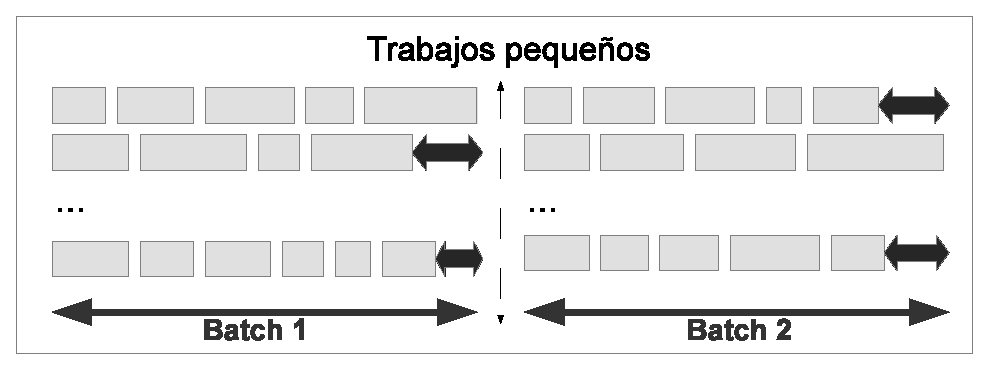
\includegraphics[scale=.75]{images/small_jobs.eps}
\caption{Ejecución en paralelo de \textit{small jobs}}
\label{fig:small_jobs}
\end{figure}

\begin{figure}[H]
\centering
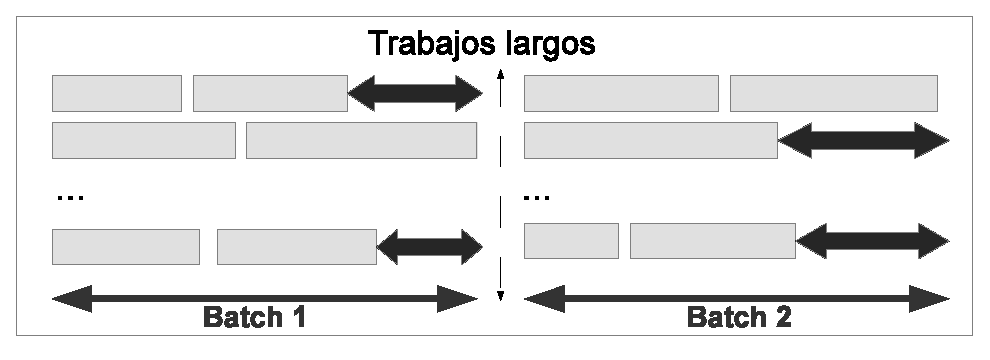
\includegraphics[scale=.75]{images/large_jobs.eps}
\caption{Ejecución en paralelo de \textit{large jobs}}
\label{fig:large_jobs}
\end{figure}



\section{Estrategia unidades de trabajo}
\label{scheduling:unidadestrabajo}
Con respecto a los esquemas explicados hasta ahora, el esquema 1TQ tiene la ventaja que no solo requiere menos control, sino que también permite a los hilos de ejecución trabajar sin pausa mientras un \textit{batch} de consultas está siendo procesado. En esta sección se propone un esquema híbrido basado en unidades de procesamiento (\textit{Processing Units}) que aproveche las ventajas de ambos enfoques. (se requiere ver el tema de bloques).
En este nuevo esquema de planificación, las consultas pasan a través de una fase en la cual cada \textit{query} es evaluada y se determina un apropiado número de unidades de procesamiento (\textit{processing units}) para poder resolver dicha consulta. Este proceso es llevado a cabo de manera similar al proceso en donde se determina la cantidad de \textit{threads} apropiados para resolver una determina transacción de lectura. Este número de unidades de procesamiento es creado y asociado a cada consulta, finalmente se guarda en una cola de unidades de trabajo. Un conjunto de \textit{threads} consumidores extraen las unidades desde la cola y las procesa independientemente. Cuando un \textit{thread} finalice el procesamiento de la unidad de trabajo actual automáticamente leerá la siguiente unidad de trabajo desde la cola. 
Generalmente lo que se hace habitualmente es estimar el número de \textit{threads} con el que se resolverá la consulta, como se muestra en la Figura \ref{fig:unit_process} en este nuevo enfoque se intenta estimar el número de unidades de trabajo con el que se resolverá cada consulta. Además, se debe controlar el acceso concurrente de los hilos de ejecución a la cola de unidades de trabajo, de tal manera que solo un thread tenga acceso exclusivo a la estructura de datos. 

\begin{figure}[!th]
\centering
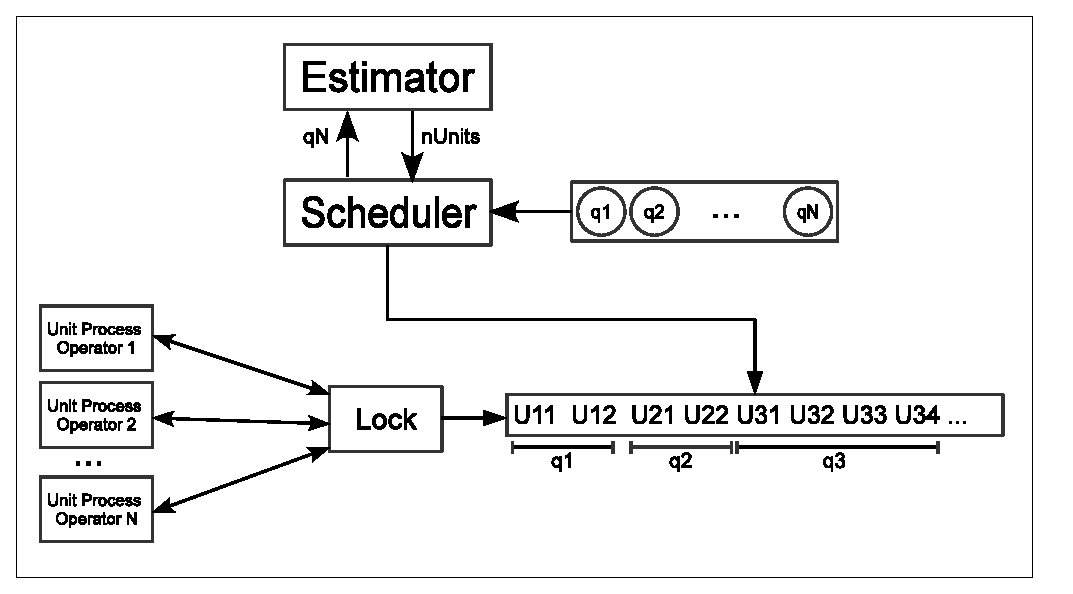
\includegraphics[scale=.75]{images/unit_process.eps}
\caption{Procesamiento de consultas utilizando unidades de trabajo}
\label{fig:unit_process}
\end{figure}

El procesamiento de cada hilo de ejecución es una versión de Wand con heap compartido (SH), adaptado de manera tal que cada unidad de trabajo es resuelta independientemente de si existen otras unidades siendo procesada al mismo tiempo o no. La única excepción es que la unidad que inicializa la consulta es siempre ejecutada antes del resto de las otras unidades de la misma consulta y la entrega de resultados se hace una vez que todas las unidades de trabajo de la \textit{query} han finalizado. Este enfoque híbrido permite reducir el tiempo perdido al final de cada \textit{batch} sin generar una importante pérdida de trabajo mientras las \textit{queries} del \textit{batch} están siendo procesadas.
